\chapter{Resultados y Discusión}
\label{cap:Resultados}

En este capítulo se presentan y discuten los resultados obtenidos por los modelos de segmentación cerebral y de segmentación de isquemia cerebral desarrollados en este trabajo. La evaluación se ha realizado sobre un subconjunto de test compuesto por tres casos representativos: un sujeto de control sin presencia de lesión y dos sujetos con lesión isquémica, correspondientes a los escenarios de isquemia transitoria e isquemia permanente. 

Cada caso dispone de 28 cortes axiales para la evaluación de la segmentación cerebral. En los casos patológicos se dispone, además, de 9 cortes con anotación específica de la región isquémica, lo que da lugar a un total de 84 cortes empleados en la evaluación cerebral y 18 cortes adicionales de lesión para la evaluación específica de isquemia. En conjunto, el análisis considera 102 imágenes de test.

Es importante precisar que la unidad principal de análisis en este capítulo es el caso completo, no el corte individual. Por este motivo, las gráficas comparativas por paciente muestran valores agregados, calculados como la media de los resultados obtenidos en todos los cortes correspondientes a cada caso. Esta decisión evita interpretar cada slice como una muestra independiente, ya que los cortes de un mismo volumen pertenecen al mismo sujeto y están anatómicamente correlacionados. No obstante, cuando resulta relevante para estudiar la variabilidad interna de cada volumen, el análisis se complementa con métricas calculadas a nivel de corte, especialmente en los apartados de explicabilidad y en la discusión de los cortes extremos.

En el caso del modelo de segmentación de isquemia, se ha aplicado un umbral de binarización de 0.8 sobre la salida probabilística del modelo. Este valor fue seleccionado previamente por ofrecer el mejor compromiso entre precisión espacial, estabilidad volumétrica y reducción de falsos positivos, tal como se observa en la Tabla~\ref{tab:comparacion_threshold}. Aunque umbrales inferiores obtienen valores de Dice ligeramente superiores, el umbral 0.8 presenta el menor error absoluto y relativo de volumen, con un error absoluto de 0.0001 ml y un error relativo del 0.86\%. Por este motivo, se priorizó este valor como punto de equilibrio entre solapamiento espacial y precisión volumétrica. La evaluación debe interpretarse como una validación exploratoria orientada a analizar el comportamiento del sistema ante distintos escenarios representativos, y no como una validación clínica definitiva sobre una cohorte amplia.

\section{Configuración experimental}
La evaluación experimental se ha diseñado con el objetivo de analizar el comportamiento de los modelos desarrollados en condiciones representativas del uso previsto de la herramienta. Para ello, se han considerado dos tareas principales: la segmentación del cerebro completo y la segmentación de regiones de isquemia cerebral. Aunque ambas tareas se abordan mediante arquitecturas basadas en U-Net, presentan niveles de dificultad distintos. La segmentación cerebral corresponde a una estructura anatómica amplia y relativamente bien delimitada, mientras que la segmentación de isquemia implica regiones más pequeñas, de borde difuso y con mayor variabilidad visual.

El conjunto de test está formado por tres casos completos. El primero corresponde a un caso de control, sin presencia de lesión, y permite evaluar la capacidad del sistema para no generar detecciones patológicas incorrectas. Los otros dos casos corresponden a sujetos con lesión isquémica, incluyendo un escenario de isquemia transitoria y otro de isquemia permanente. Esta selección permite cubrir tres situaciones relevantes para el análisis: ausencia de lesión, lesión de menor definición e intensidad, y lesión más estable y claramente visible.

Para cada caso se han evaluado las máscaras generadas por el modelo frente a las segmentaciones manuales disponibles. En la tarea de segmentación cerebral se han utilizado los 28 cortes de cada volumen, dando lugar a 84 cortes evaluados. En la tarea de segmentación de isquemia se han analizado los cortes anotados con información específica de lesión, correspondientes a los casos patológicos. Además, el caso de control se ha incluido en la evaluación de isquemia para comprobar que el modelo mantiene un comportamiento conservador en ausencia de patología.

Las métricas cuantitativas empleadas han sido el coeficiente Dice, la intersección sobre la unión o IoU, el error absoluto de volumen, el error relativo y el porcentaje de acierto volumétrico. Dice e IoU permiten medir el solapamiento espacial entre la máscara predicha y la máscara de referencia, mientras que las métricas volumétricas permiten valorar si la herramienta estima de forma adecuada la magnitud de la estructura segmentada. Esta segunda dimensión resulta especialmente relevante para el objetivo del proyecto, ya que la herramienta no solo busca generar máscaras visuales, sino también cuantificar automáticamente regiones anatómicas o patológicas.

Las gráficas por paciente representan la media de los valores obtenidos en los slices de cada sujeto. Esta forma de presentación permite comparar de manera clara el comportamiento del modelo entre casos.

Además del análisis cuantitativo, se ha realizado una evaluación cualitativa de las segmentaciones generadas. Este análisis visual resulta necesario en el contexto de la imagen biomédica, ya que las métricas de solapamiento pueden penalizar de forma intensa pequeñas diferencias en los bordes, especialmente cuando las regiones segmentadas son pequeñas o presentan límites ambiguos. Por este motivo, la interpretación de los resultados combina métricas numéricas, comparación visual de máscaras y análisis de coherencia espacial mediante técnicas de explicabilidad.

Finalmente, para el modelo de isquemia se ha estudiado el impacto del umbral de binarización aplicado sobre la salida probabilística. En este capítulo se presentan los resultados correspondientes al umbral 0.8, seleccionado por ofrecer un equilibrio adecuado entre detección de lesión y reducción de falsos positivos. Esta decisión es especialmente importante en la segmentación de isquemia, donde valores de umbral más bajos pueden aumentar la sensibilidad, pero también producir sobresegmentaciones en regiones de intensidad intermedia.

\section{Resultados en segmentación cerebral}
La primera tarea evaluada corresponde a la segmentación del cerebro completo. Esta tarea constituye una etapa fundamental dentro del flujo de análisis, ya que permite aislar la región anatómica de interés y proporciona una base sobre la que posteriormente pueden calcularse medidas volumétricas o aplicarse procedimientos específicos de análisis de lesión.

\subsection{Resultados cuantitativos}
La Tabla~\ref{tab:metricas_cerebro} resume las métricas obtenidas por el modelo de segmentación cerebral sobre los casos de test. Los resultados muestran un rendimiento elevado y estable, con un coeficiente Dice 3D medio de $0.973 \pm 0.001$ y una IoU 3D media de $0.947 \pm 0.002$. Estos valores indican un alto grado de solapamiento entre las máscaras predichas y las segmentaciones de referencia.


\begin{table}[h]
\centering
\caption{Resumen de métricas del modelo de segmentación cerebral}
\begin{tabular}{lc}
\hline
\textbf{Métrica} & \textbf{Valor} \\
\hline
Error absoluto medio (ml) & $0.007 \pm 0.004$ \\
Error relativo medio (\%) & $1.56 \pm 0.90$ \\
Acierto medio (\%) & $98.44$ \\
Coeficiente Dice 3D & $0.973 \pm 0.001$ \\
IoU 3D & $0.947 \pm 0.002$ \\
\hline
\end{tabular}
\label{tab:metricas_cerebro}
\end{table}

Desde el punto de vista volumétrico, el modelo obtiene un error absoluto medio de $0.007$ ml y un error relativo medio del $1.56\%$. Estos valores muestran que la segmentación automática no solo reproduce adecuadamente la forma espacial del cerebro, sino que también conserva de manera precisa su volumen total. Este aspecto resulta relevante para la herramienta desarrollada, ya que una estimación volumétrica estable es necesaria para que los resultados puedan ser utilizados posteriormente en tareas de cuantificación biomédica.

En la Figura~\ref{fig:dice_paciente_cerebro} se representan los valores medios del coeficiente Dice obtenidos para cada caso. Cada punto corresponde a la media de los valores calculados sobre los cortes del volumen correspondiente. Como se observa, el rendimiento se mantiene estable entre los tres casos evaluados, sin caídas relevantes asociadas a la presencia o ausencia de lesión isquémica. Este comportamiento sugiere que el modelo de cerebro aprende una representación anatómica robusta y no depende de forma significativa del estado patológico del sujeto.

\begin{figure}[h]
    \centering
    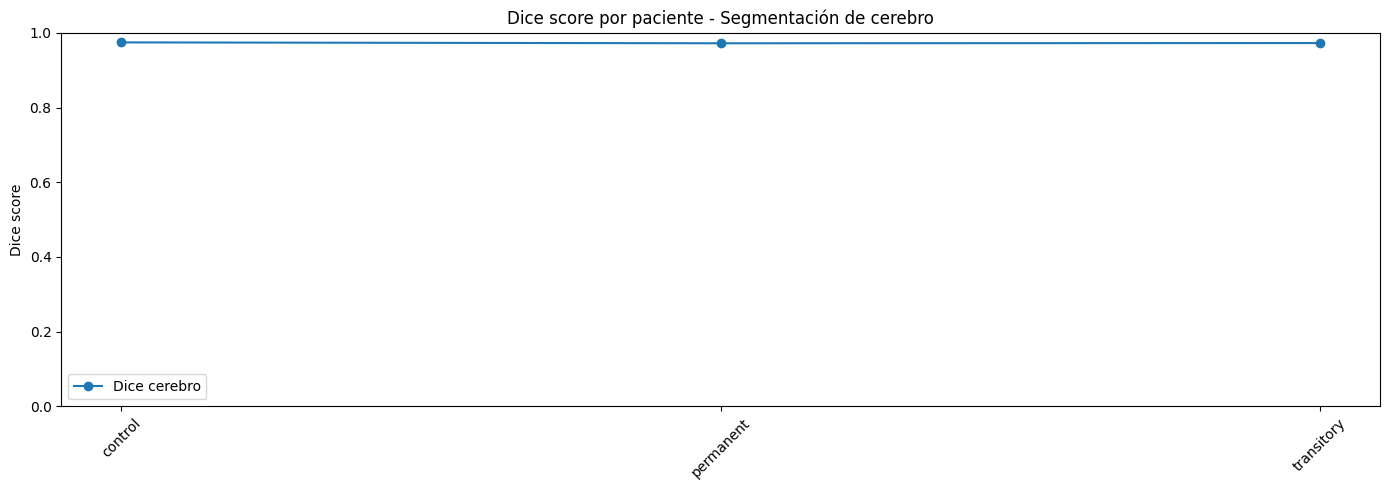
\includegraphics[width=1\textwidth]{Imagenes/Plots/dice_paciente_cerebro.png}
    \caption{Evolución del coeficiente Dice por Caso}
    \label{fig:dice_paciente_cerebro}
\end{figure}

La Figura~\ref{fig:volumen_cerebro} compara el volumen cerebral estimado por el modelo con el volumen obtenido a partir de la segmentación manual. La proximidad entre ambos valores confirma que las diferencias observadas son reducidas y que el modelo mantiene una estimación volumétrica coherente en los tres casos. Esta estabilidad es especialmente importante porque pequeñas desviaciones sistemáticas en la segmentación del cerebro podrían propagarse a etapas posteriores del análisis.

\begin{figure}[h]
    \centering
    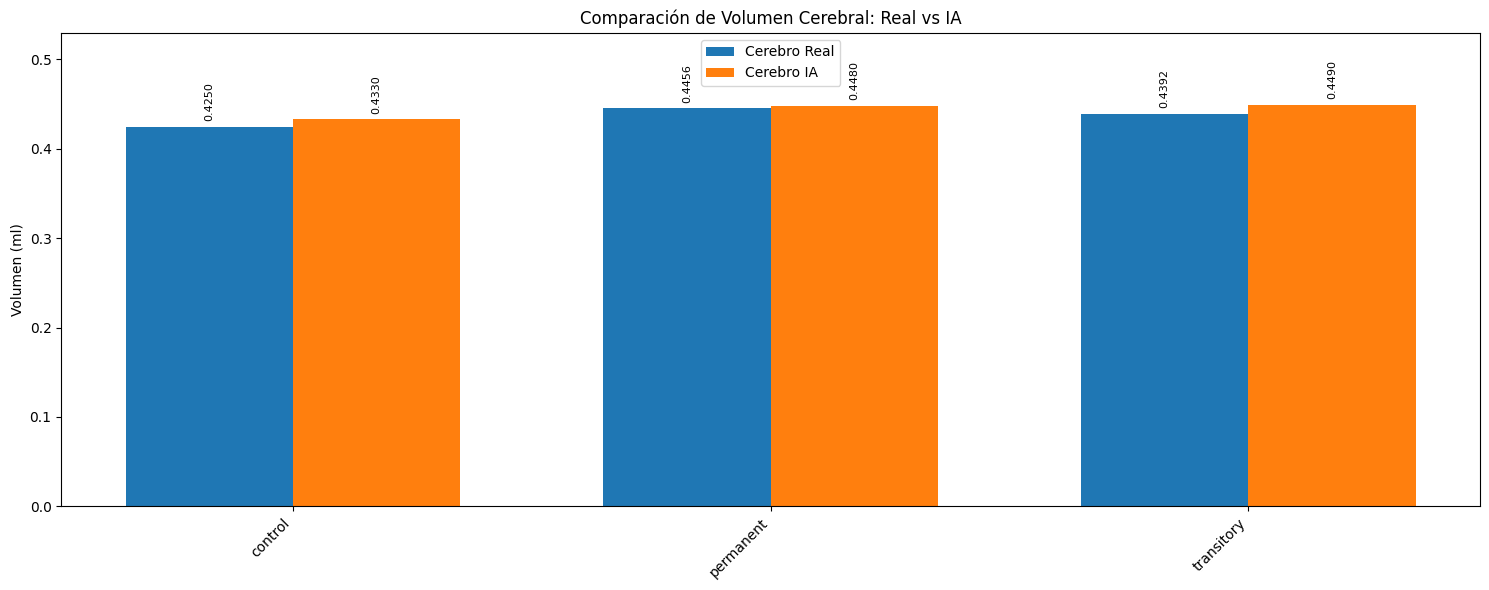
\includegraphics[width=1\textwidth]{Imagenes/Plots/volumen_cerebro.png}
    \caption{Evolución del coeficiente Dice por caso}
    \label{fig:volumen_cerebro}
\end{figure}

En conjunto, los resultados cuantitativos muestran que el modelo de segmentación cerebral alcanza un comportamiento preciso, estable y adecuado para su integración en la herramienta desarrollada. La baja variabilidad entre casos indica que el modelo generaliza correctamente dentro del subconjunto de evaluación utilizado, al menos para los escenarios representativos considerados en este trabajo.


\subsection{Análisis cualitativo}
Con el objetivo de complementar la evaluación cuantitativa, se ha realizado un análisis visual de las máscaras generadas por el modelo. La Figura~\ref{fig:cualitativo_cerebro} muestra ejemplos representativos de la segmentación cerebral obtenida en los distintos casos evaluados. En cada ejemplo se compara la imagen original, la máscara de referencia y la máscara predicha por el modelo.


\begin{figure}[h]
    \centering
    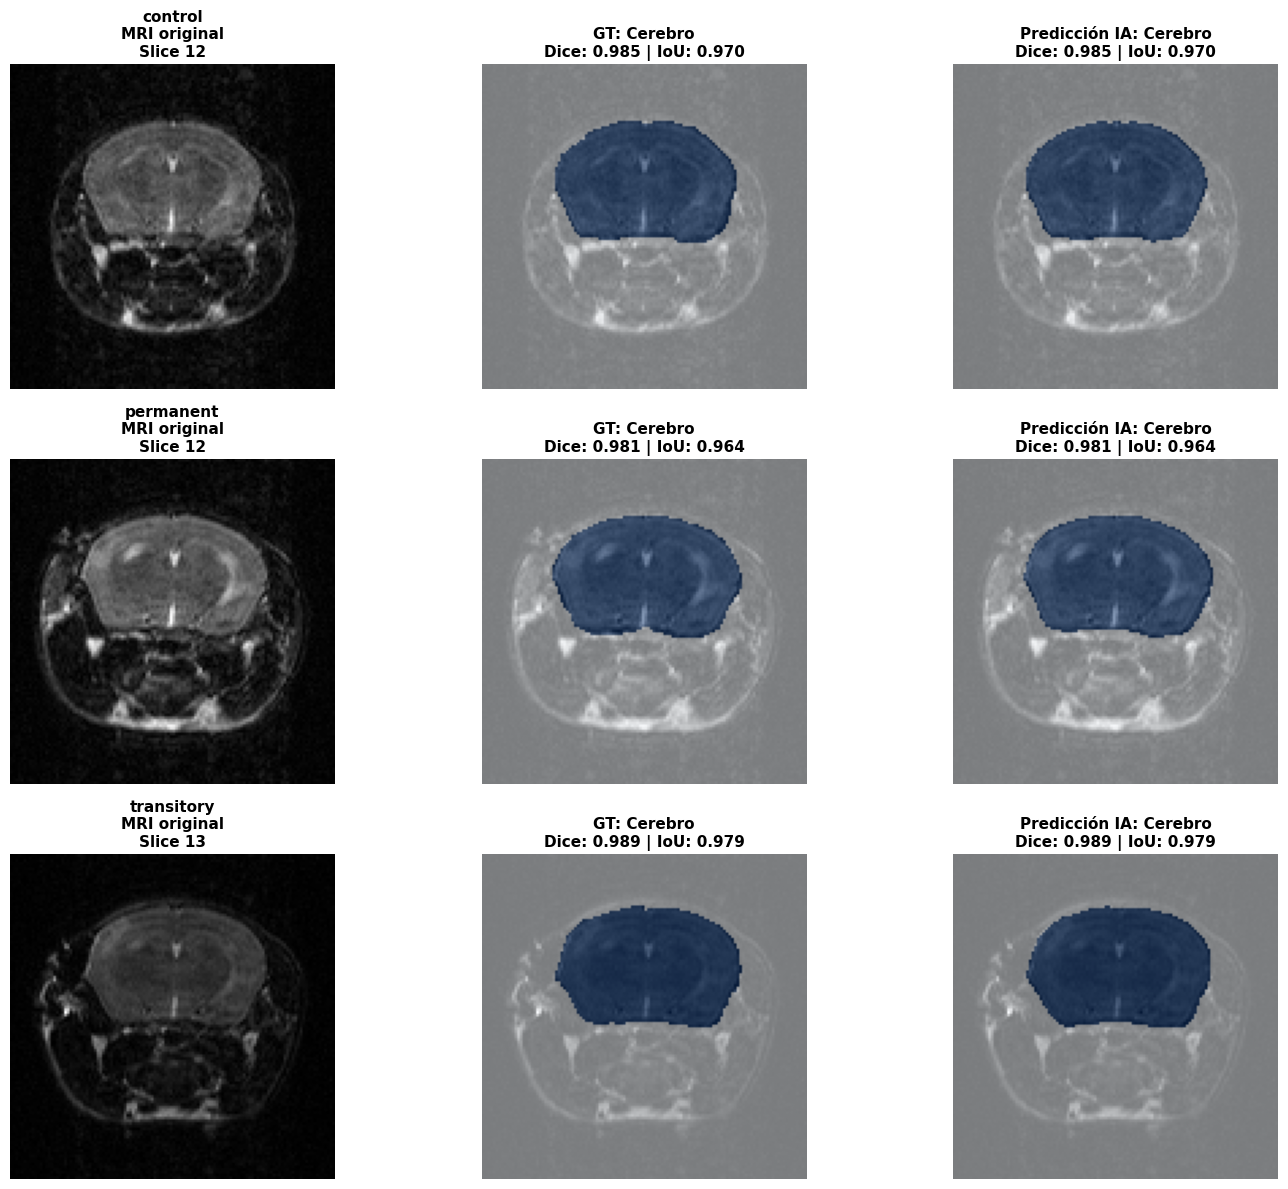
\includegraphics[width=1\textwidth]{Imagenes/Plots/cualitativo_cerebro.png}
    \caption{Ejemplos cualitativos de segmentación de isquemia en distintos escenarios}
    \label{fig:cualitativo_cerebro}
\end{figure}

A nivel visual, las máscaras generadas presentan una delimitación coherente del contorno cerebral. El modelo conserva forma de la estructura y no presenta artefactos fuera del área esperada. Este comportamiento es consistente con los valores elevados de Dice e IoU observados en el análisis cuantitativo.

Las principales  se concentrdiscrepanciasan en los cortes extremos de los casos, donde las slices contienen ruido y son menos definida. Estos cortes no se han tenido en cuenta, ya que en un entorno de investigación son descartados por su baja calidad e interés, ya que no forman parte de la anatomía cerebral relevante para el análisis de la isquemia cerebral.

En los cortes centrales, la segmentación es precisa y la estructura está bien definida, presentando bordes incluso más ajustados que la segmentación manual. Esto indica que el modelo es capaz de identificar de manera estable la región cerebral principal, incluso en presencia de variaciones de intensidad propias de la resonancia magnética.

\subsection{Resultados de explicabilidad en la segmentación de cerebro}
Además de evaluar la calidad de las máscaras generadas, se aplicaron técnicas de explicabilidad con el objetivo de analizar la coherencia espacial de las regiones utilizadas por el modelo durante la predicción. Este análisis no pretende sustituir a las métricas clásicas de segmentación, sino complementarlas mediante una evaluación del comportamiento interno del modelo. Esto es especialmente importante en un pipeline aplicado a la investigación biomédica. 

El análisis se realizó sobre 84 cortes pertenecientes a tres casos distintos. No obstante, durante la interpretación de los resultados se observó que los cortes extremos de cada volumen presentan un comportamiento diferente al de los cortes centrales. En estas zonas, la presencia de tejido cerebral es reducida o incluso inexistente en la máscara de referencia, lo que afecta negativamente a métricas como Dice e IoU y puede producir valores poco representativos. Por este motivo, los resultados se analizaron distinguiendo entre cortes interiores y cortes extremos.

En el conjunto completo de cortes analizados, el modelo obtuvo un Dice medio de 0,802 y un IoU medio de 0,774. Sin embargo, al considerar únicamente los cortes interiores, más representativos de la tarea principal de segmentación cerebral, el rendimiento aumentó notablemente, alcanzando un Dice medio de 0,969 y un IoU medio de 0,940. Esta diferencia indica que la reducción del rendimiento global se debe principalmente a los cortes de borde, donde la región anatómica objetivo es pequeña o ambigua, y no a un fallo sistemático del modelo en la segmentación del cerebro.

\begin{table}[H]
\centering
\caption{Rendimiento medio del modelo de segmentación cerebral en los cortes analizados para explicabilidad.}
\label{tab:rendimiento_xai_cerebro}
\begin{tabular}{lccc}
\toprule
\textbf{Conjunto de cortes} & \textbf{N} & \textbf{Dice medio} & \textbf{IoU medio} \\
\midrule
Todos los cortes & 84 & 0,802 & 0,774 \\
Cortes interiores & 66 & 0,969 & 0,940 \\
Cortes extremos & 18 & 0,189 & 0,174 \\
\bottomrule
\end{tabular}
\end{table}

La Figura~\ref{fig:xai_cerebro_ejemplo_bueno} muestra ejemplos representativos de cortes interiores en los que el modelo obtiene una segmentación cerebral precisa. En cada fila se presenta la imagen original, la máscara de referencia, la máscara predicha, los mapas de relevancia generados por Grad-CAM, Grad-CAM++ e Integrated Gradients, y la curva de eliminación normalizada asociada.

\begin{figure}[H]
    \centering
    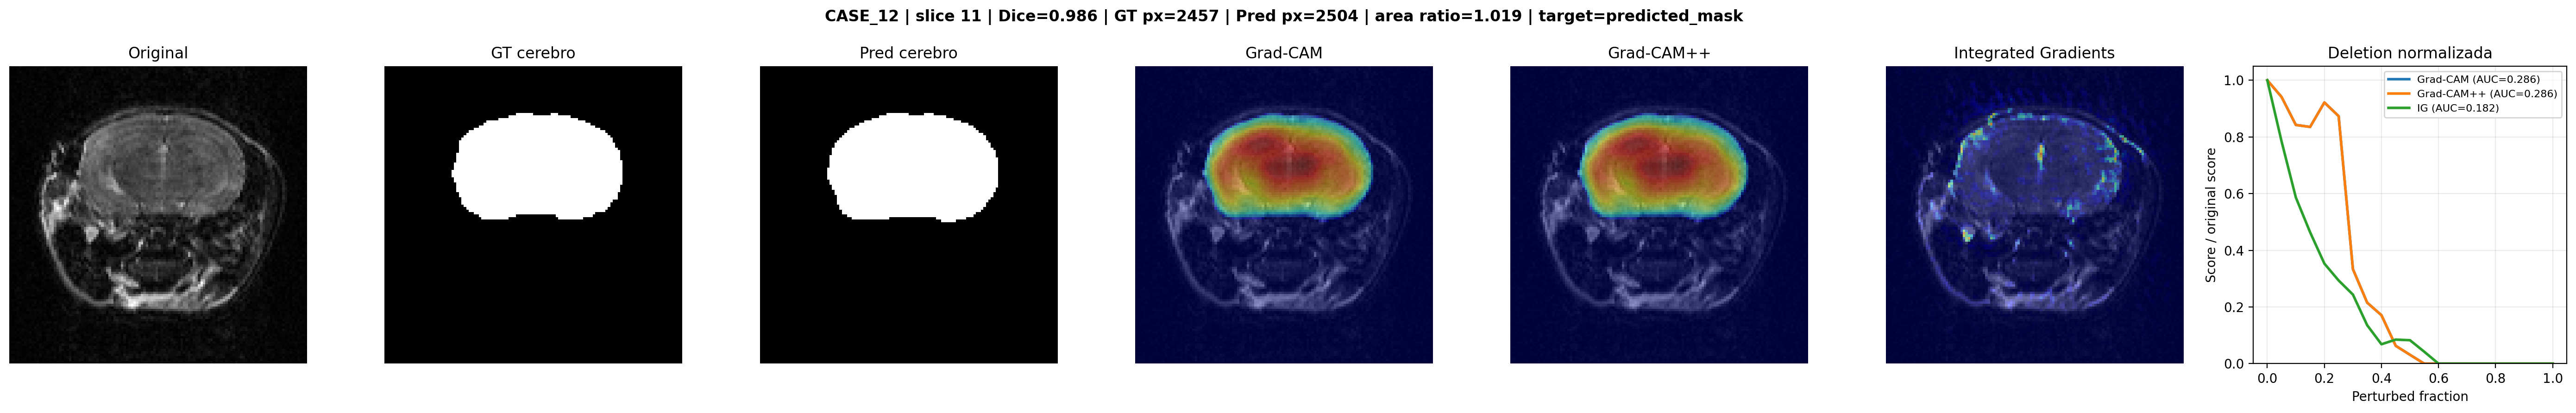
\includegraphics[width=\textwidth]{Imagenes/XAI_Cerebro/good_brain_segmentation/CASE_12_slice_011.png}
    \caption{Ejemplo cualitativo de explicabilidad aplicado al modelo de segmentación cerebral. Se muestra la imagen original, la máscara manual, la máscara predicha, los mapas obtenidos mediante Grad-CAM, Grad-CAM++ e Integrated Gradients, y la curva de eliminación normalizada.}
    \label{fig:xai_cerebro_ejemplo_bueno}
\end{figure}

En estos ejemplos, la máscara predicha presenta un alto grado de solapamiento con la segmentación manual, con valores Dice próximos a 1. Esta coincidencia entre la evaluación cuantitativa y la visualización de los mapas de relevancia refuerza la interpretación de que, en los cortes representativos del volumen, el modelo realiza una segmentación estable y espacialmente coherente. Además, tanto Grad-CAM como Grad-CAM++ producen mapas suaves y continuos, lo que facilita su interpretación visual en el contexto de una tarea de segmentación anatómica.

Integrated Gradients, por el contrario, muestra un patrón más localizado y disperso. En lugar de generar una región amplia de activación sobre todo el cerebro, tiende a resaltar puntos concretos, bordes o zonas de mayor variación de intensidad. Este comportamiento puede resultar menos intuitivo desde el punto de vista visual, pero es coherente con los resultados cuantitativos obtenidos en las métricas de eliminación, donde este método mostró una mayor sensibilidad al retirar las regiones consideradas relevantes. Por tanto, Integrated Gradients parece identificar zonas críticas para la predicción, aunque su representación sea menos directa que la obtenida mediante Grad-CAM o Grad-CAM++.

Las curvas de eliminación normalizada permiten complementar esta interpretación visual. En ellas se observa cómo varía la puntuación del modelo al perturbar progresivamente las regiones identificadas como relevantes por cada método. En los casos con buena segmentación, la eliminación de las zonas destacadas provoca una caída progresiva de la puntuación, lo que indica que dichas regiones tienen una influencia real sobre la salida del modelo. Esta relación entre mapas de relevancia y caída del score aporta una medida adicional de fidelidad de las explicaciones.

No obstante, el análisis cualitativo también evidencia ciertas limitaciones. En los cortes extremos del volumen, la interpretación de los mapas resulta menos estable. En algunos de estos cortes, la máscara manual contiene muy poca región cerebral o incluso ningún píxel etiquetado, mientras que la imagen todavía puede presentar estructuras anatómicas residuales. En estos casos, el modelo puede generar una predicción parcial de cerebro, lo que conduce a valores Dice nulos o muy bajos y a ratios de área no representativos. Por ello, estos cortes no deben interpretarse del mismo modo que los cortes interiores.

Esta diferencia justifica la separación realizada entre cortes interiores y cortes extremos en el análisis cuantitativo. Los cortes interiores permiten evaluar el comportamiento del modelo en las regiones donde la estructura cerebral está claramente presente, mientras que los cortes de borde reflejan situaciones más ambiguas, condicionadas tanto por la anatomía visible como por el criterio de anotación manual. En consecuencia, las explicaciones obtenidas en cortes extremos deben entenderse como una herramienta para estudiar el comportamiento del modelo ante casos límite, no como una medida directa de buen funcionamiento.

En conjunto, el análisis cualitativo de los mapas de relevancia muestra que, en los cortes representativos de la estructura cerebral, las explicaciones son coherentes con la segmentación obtenida. Grad-CAM y Grad-CAM++ ofrecen visualizaciones más suaves y anatómicamente interpretables, mientras que Integrated Gradients proporciona una explicación más sensible a regiones concretas de la imagen. La combinación de estos métodos permite analizar el modelo desde perspectivas complementarias y aporta información útil sobre la relación entre la imagen de entrada, la máscara predicha y las regiones que influyen en la predicción.

Una vez caracterizado el comportamiento del modelo, se evaluó la fidelidad de las explicaciones mediante métricas basadas en perturbación. En particular, se utilizaron curvas de eliminación e inserción, así como sus variantes MoRF y LeRF. En las curvas de eliminación, se eliminan progresivamente las regiones más relevantes según el mapa de explicación; por tanto, un valor bajo de \textit{Deletion AUC} indica que la explicación identifica regiones importantes para la predicción. En cambio, en las curvas de inserción, valores altos de \textit{Insertion AUC} indican que las regiones destacadas por el método permiten reconstruir progresivamente la activación del modelo.

La Tabla~\ref{tab:xai_cerebro_metricas} resume los resultados medios obtenidos para Grad-CAM, Grad-CAM++ e Integrated Gradients. La sensibilidad por oclusión se empleó como análisis complementario, pero no se incluye en esta tabla al no calcular las mismas métricas agregadas que los métodos basados en mapas de relevancia.

\begin{table}[H]
\centering
\caption{Resumen cuantitativo de las métricas de fidelidad para los métodos de explicabilidad aplicados al modelo de segmentación cerebral.}
\label{tab:xai_cerebro_metricas}
\resizebox{\textwidth}{!}{%
\begin{tabular}{lccccc}
\toprule
\textbf{Método} & \textbf{Deletion AUC} $\downarrow$ & \textbf{Insertion AUC} $\uparrow$ & \textbf{LeRF AUC} $\uparrow$ & \textbf{AOPC} $\uparrow$ & \textbf{AOPC norm.} $\uparrow$ \\
\midrule
Grad-CAM & 0,264 & 0,712 & 0,755 & 0,753 & 0,761 \\
Grad-CAM++ & 0,304 & \textbf{0,795} & \textbf{0,807} & 0,714 & 0,721 \\
Integrated Gradients & \textbf{0,102} & 0,755 & 0,721 & \textbf{0,914} & \textbf{0,923} \\
\bottomrule
\end{tabular}%
}
\end{table}
Los resultados muestran que Integrated Gradients obtuvo el mejor comportamiento en las métricas basadas en eliminación, con un \textit{Deletion AUC} medio de 0,102 y un \textit{AOPC} normalizado de 0,923. Esto indica que las regiones identificadas como relevantes por este método tienen una influencia directa sobre la predicción del modelo, ya que su eliminación provoca una reducción rápida de la puntuación asociada a la segmentación cerebral.

Por otro lado, Grad-CAM++ presentó los mejores valores en las métricas de inserción y LeRF, con un \textit{Insertion AUC} medio de 0,795 y un \textit{LeRF AUC} medio de 0,807. Este resultado sugiere que las regiones resaltadas por Grad-CAM++ contienen información suficiente para reconstruir progresivamente la predicción del modelo, y que las zonas consideradas menos relevantes afectan en menor medida a la salida cuando se eliminan en primer lugar.

El comportamiento de las curvas de perturbación refuerza esta interpretación. En el caso de Integrated Gradients, al eliminar el 25\% de los píxeles considerados más relevantes, la puntuación media del modelo descendió hasta 0,097. En cambio, para Grad-CAM y Grad-CAM++, la puntuación en ese mismo punto fue de 0,663 y 0,750, respectivamente. Esto sugiere que Integrated Gradients produce mapas más focalizados en regiones críticas para la predicción, mientras que Grad-CAM y Grad-CAM++ generan explicaciones más distribuidas espacialmente.


En conjunto, los resultados de explicabilidad no deben interpretarse como una validación clínica independiente del modelo, sino como una herramienta complementaria para analizar su comportamiento. Las métricas cuantitativas indican que las regiones destacadas por los métodos XAI influyen de forma significativa en la predicción, especialmente en el caso de Integrated Gradients. Asimismo, Grad-CAM++ aporta una visualización útil para interpretar la reconstrucción progresiva de la evidencia visual. Por tanto, la combinación de estos métodos permite obtener una visión más completa del proceso de segmentación realizado por el modelo.

\section{Resultados en segmentación de isquemia}
A continuación, se presentan los resultados obtenidos en la tarea de segmentación de las regiones de lesión por isquemia cerebral, la cual, por razones que se describirán en la siguiente sección, supone un problema más complejo que la segmentación del órgano sano. Para ello, al igual que en el modelo de cerebro, se han evaluado varias configuraciones de arquitecturas \textit{U-Net}, utilizando las métricas descritas anteriormente.

\subsection{Resultados cuantitativos} 
\begin{table}[h]
\centering
\caption{Resumen de métricas del modelo de segmentación de isquemia}
\begin{tabular}{lc}
\hline
\textbf{Métrica} & \textbf{Valor} \\
\hline
Error absoluto medio (ml) & $0.001 \pm 0.001$ \\
Error relativo medio (\%) & $7.41 \pm 2.64$ \\
Acierto medio (\%) & $92.59$ \\
Coeficiente Dice 3D & $0.820 \pm 0.157$ \\
IoU 3D & $0.717 \pm 0.246$ \\
\hline
\end{tabular}
\label{tab:metricas_isquemia}
\end{table}

En la Figura \ref{fig:dice_paciente_isquemia} se representan los valores del coeficiente Dice obtenidos para cada uno de los casos evaluados en la tarea de segmentación de isquemia.

\begin{figure}[h]
    \centering
    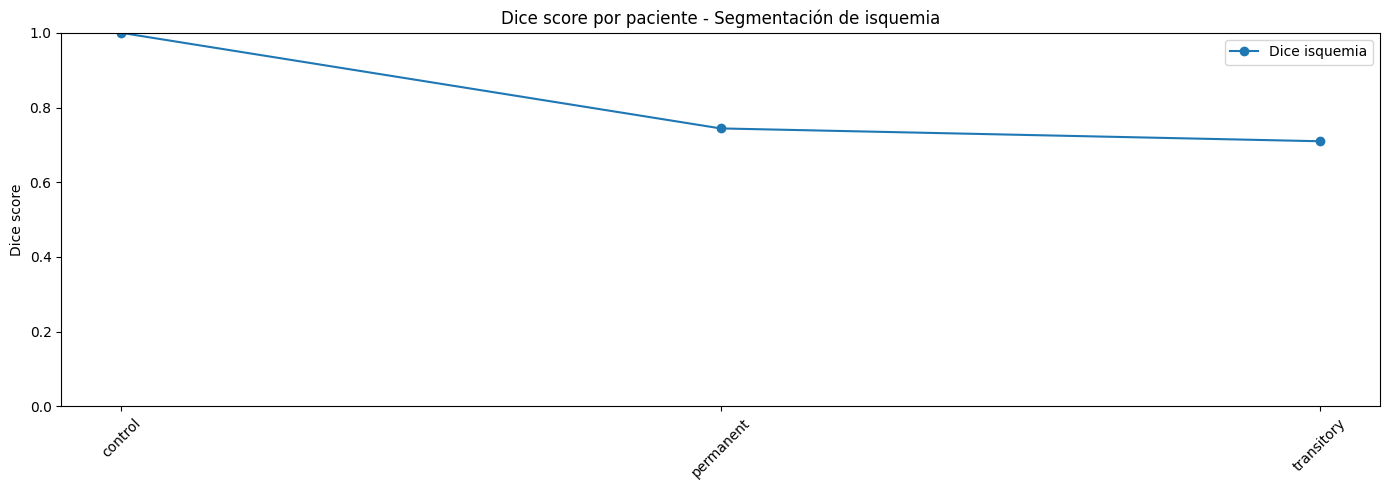
\includegraphics[width=1\textwidth]{Imagenes/Plots/dice_paciente_isquemia.png}
    \caption{Evolución del coeficiente Dice por Caso}
    \label{fig:dice_paciente_isquemia}
\end{figure}
En el caso de control, donde no existe presencia de lesión, el modelo obtiene un valor de Dice igual a 1, lo que indica una coincidencia perfecta entre la predicción y la máscara de referencia al no detectar regiones patológicas. En los casos con presencia de isquemia, los valores de Dice se sitúan en torno a 0.8, lo que refleja un alto grado de solapamiento entre la segmentación automática y la manual, aunque con discrepancias en las zonas de transición y en la delimitación de los bordes.

De manera general, los resultados obtenidos muestran un valor de \textit{coeficiente Dice} inferiores y con mayor variabilidad frente al modelo de cerebro. El error relativo también presenta una ligera degradación respecto al caso base.

Estas diferencias son notables a lo largo de todas las configuraciones y casos analizados, lo que sugiere que la limitación no reside únicamente en el modelo, sino en la naturaleza del problema abordado.

\subsection{Naturaleza del problema y subjetividad}
A diferencia de la segmentación del cerebro, el cual está claramente delimitado por el cráneo y el espacio subcranoideo, debido a las características anatómicas propias de las lesiones de isquemia cerebral, el proceso de segmentación constituye un problema complejo y altamente subjetivo, cuya interpretación puede variar significativamente entre distintos profesionales, tal y como respalda el\textit{ ICTS BioImagen Complutense}.

Concretamente, las lesiones presentan las siguientes características visibles en cada corte de la IRM afectado:
 \begin{itemize}
    \item Borde difuminado.
    \item Gradientes de intensidad entre tejido sano y afectado.
    \item Zonas intermedias en las que la clasificación no es clara.
    \item Ruido y artefactos propios de la resonancia magnética nuclear.
\end{itemize}
Como consecuencia, la delimitación manual de estas regiones depende del criterio del experto que realiza la medición, lo que introduce una alta variabilidad en los datos recogidos entre observadores y estudios.
La anotación manual está afectada por incertidumbre en la frontera de la lesión, y penaliza las métricas de solapamiento, por lo que el\textbf{ \textit{ground truth}} utilizado durante el entrenamiento y la evaluación del modelo debe analizarse con concordancia a una referencia experta operativa.

\subsection{Interpretación de métricas}
Teniendo en cuenta esta problemática, los valores obtenidos en las métricas deben interpretarse con cautela. Por este motivo, ha sido necesaria una validación adicional por parte de profesionales del \textit{ ICTS BioImagen Complutense}, con el fin de obtener un veredicto más fiable y ajustado a la realidad clínica. Un \textit{valor Dice} inferior en comparación al modelo de segmentación cerebral no implica necesariamente un menor rendimiento del modelo, sino que refleja la variabilidad técnica del proceso.

Pequeñas variaciones en la delimitación de la zona afectada, producen cambios significativos en el \textit{valor Dice}, por lo que el modelo puede estar generando segmentaciones coherentes desde el punto de vista clínico aún cuando la métrica no alcance los valores óptimos.

En este punto, resulta especialmente relevante considerar el criterio aportado por los profesionales del\textit{  ICTS BioImagen Complutense}, quienes señalan que la validez de las segmentaciones no dependen únicamente de precisión absoluta sino de la robustez en el comportamiento del modelo. Es decir, una ligera sobreestimación o subestimación sistemática en los volúmenes segmentados puede considerarse válida siempre que la desviación sea consistente entre casos y no introduzca artefactos incoherentes, como cortes intermedios vacíos o la detección de regiones incompatibles con la morfología de la isquemia. 

Tal y como se observa en la Figura \ref{fig:volumen_isquemia}, las diferencias en los volúmenes estimados se mantienen en rangos  consistentes respecto al \textit{ground truth}. Este comportamiento sugiere que el modelo presenta una desviación sistemática controlada, alineada con los criterios de robustez definidos por el centro de Bioimagen.

\begin{figure}[h]
    \centering
    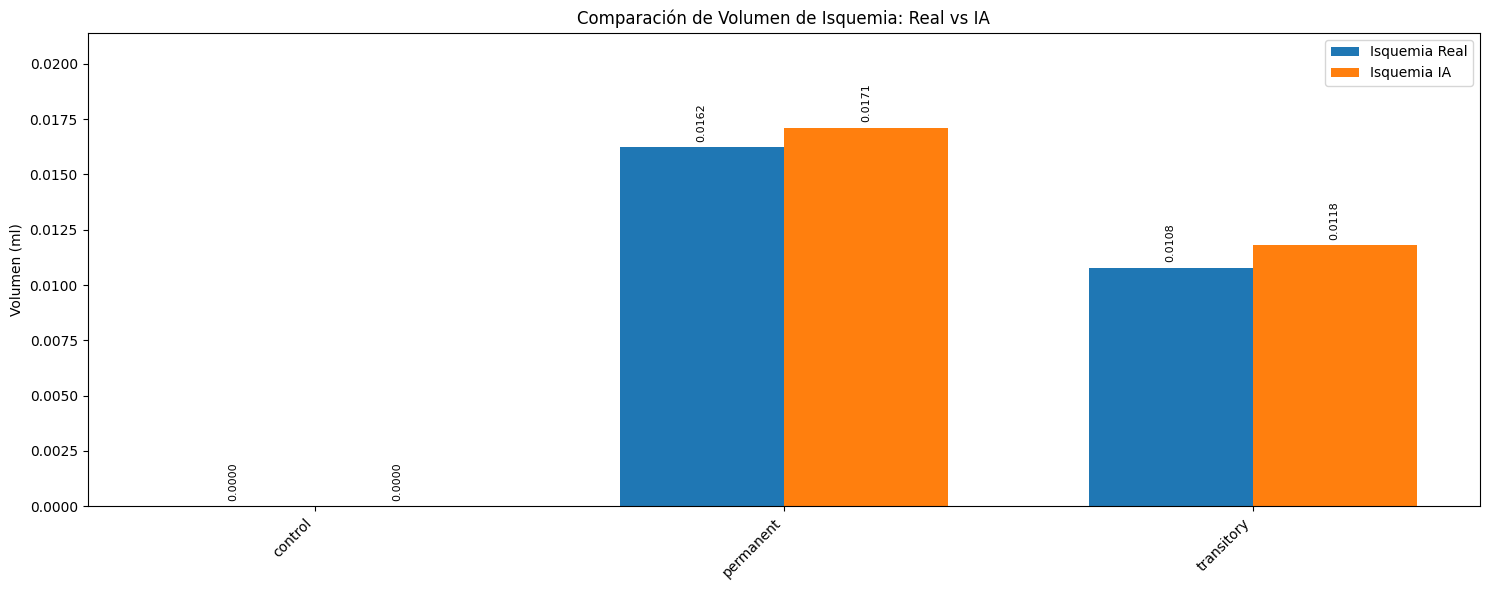
\includegraphics[width=1\textwidth]{Imagenes/Plots/volumen_isquemia.png}
    \caption{Evolución del coeficiente Dice por caso}
    \label{fig:volumen_isquemia}
\end{figure}

\subsection{Impacto del threshold}
Uno de los factores clave en la calidad de la segmentación es el umbral de decisión aplicado sobre la salida del modelo:
Valores de umbral bajos tienden a producir segmentaciones más extensas, incrementando la detección de posibles zonas afectadas, pero también introduciendo falsos positivos. 
Por lo contrario, umbrales altos generan segmentaciones más conservadoras, generando posibles omisiones de zonas de baja hiperintensidad.

Este comportamiento es especialmente crítico en el caso de la isquemia, donde las regiones ambiguas son frecuentes. Por ello, la elección del umbral óptimo depende en gran medida del criterio clínico y del uso final de la herramienta.

\subsection{Análisis cualitativo}
Con el objetivo de complementar el análisis cuantitativo presentado anteriormente, se ha realizado una evaluación cualitativa de las segmentaciones obtenidas en los casos de isquemia cerebral, prestando especial atención al comportamiento del modelo en regiones de alta ambigüedad.

\begin{figure}[h]
    \centering
    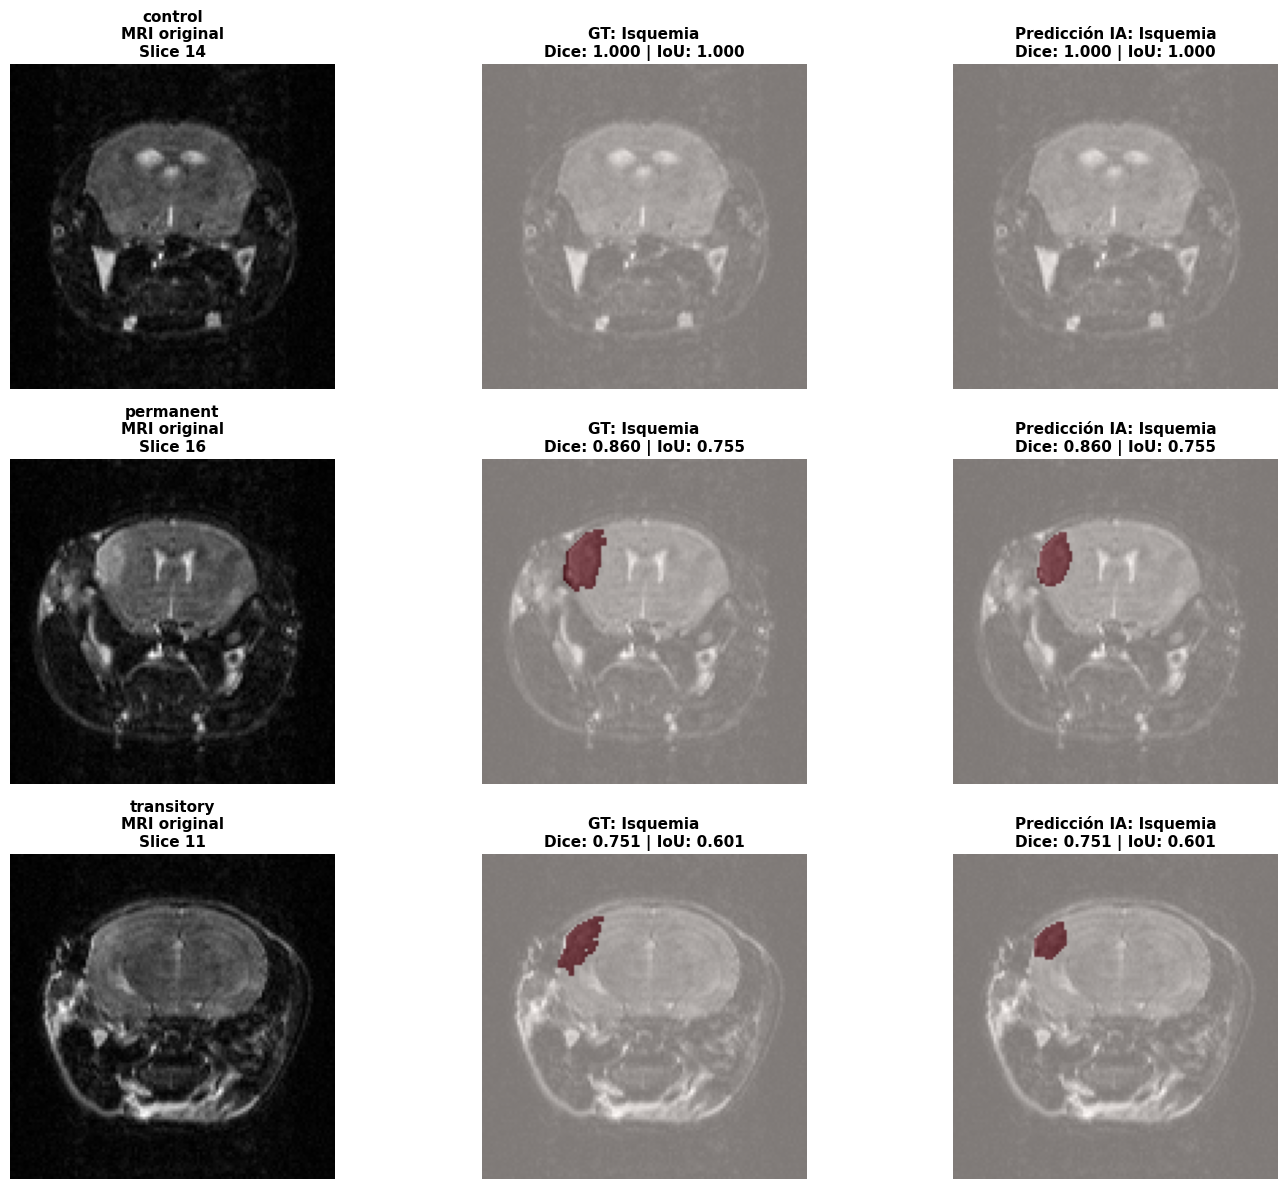
\includegraphics[width=1\textwidth]{Imagenes/Plots/cualitativo_isquemia.png}
    \caption{Ejemplos cualitativos de segmentación de isquemia en distintos escenarios}
    \label{fig:cualitativo_isquemia}
\end{figure}
La Figura \ref{fig:cualitativo_isquemia} muestra ejemplos representativos de segmentación correspondientes a los tres casos estudiados. En cada uno de ellos se comparan la máscara manual (GT), y la predicción generada por el modelo.

En el caso de control, el modelo presenta un comportamiento óptimo, con una correspondencia exacta entre la predicción y la ausencia de lesión. Este resultado confirma la capacidad del modelo para no generar falsos positivos en ausencia de patología.

En el caso de isquemia permanente, se obtiene un coeficiente Dice de 0.86 y un IoU de 0.755. A nivel visual, la predicción del modelo muestra una delimitación más homogénea y consistente de la región afectada en comparación con la máscara manual, la cual presenta bordes más irregulares. Este comportamiento sugiere que el modelo no solo reproduce la anotación, sino que puede aportar una segmentación más regular en regiones donde el ground truth es ambiguo.

Por último, en el caso de isquemia transitoria, se obtienen valores inferiores (Dice de 0.751 e IoU de 0.601), lo cual es coherente con la menor definición de la lesión. En este tipo de casos, la baja intensidad de la zona hiperintensa de la isquemia hacen que su selección manual sea compleja, intruduciendo un valor de subjetividad elevado. Sin embargo, el modelo consigue destacar exitosamente la zona más afectada pese a que el caso puede parecerse mucho a un caso de control.

En conjunto, estos resultados cualitativos refuerzan la interpretación de las métricas cuantitativas, evidenciando que las diferencias observadas en los valores de Dice no responden únicamente al rendimiento del modelo, sino también a la complejidad intrínseca de cada caso y a la variabilidad presente en las anotaciones de referencia.

Se ha observado que, debido a la mayor sensibilidad del modelo, en ocasiones se ha conseguido identificar regiones desapercibidas a criterio manual, así como de segmentar de forma más homogénea ciertas zonas de transición. Estos resultados sugieren que el modelo no solo reproduce el comportamiento humano, sino que, en determinados escenarios, puede ser una herramienta útil para mejorar la consistencia del proceso.

En segundo lugar, en las zonas de transición entre tejido sano y tejido afectado, el modelo muestra una mayor estabilidad en la delimitación de los bordes, proporcionando segmentaciones más suaves y menos fragmentadas. Este aspecto resulta especialmente relevante en el contexto de la isquemia, donde los gradientes de intensidad dificultan la definición de un límite claro.

Por otro lado, también se han identificado casos en los que el modelo presenta una ligera sobreestimación de las regiones afectadas, especialmente en áreas con intensidades intermedias. No obstante, tal y como se ha discutido previamente, este comportamiento puede considerarse aceptable siempre que se mantenga de forma consistente y no introduzca estructuras incompatibles con la morfología esperada de la lesión.

Finalmente, en los casos más complejos, el modelo muestra limitaciones similares a las de la segmentación manual, lo que refuerza la idea de que la dificultad reside en la propia naturaleza de la imagen y no exclusivamente en el enfoque empleado.

En conjunto, el análisis cualitativo respalda los resultados cuantitativos obtenidos, evidenciando que el modelo produce segmentaciones coherentes y clínicamente plausibles, incluso en aquellos casos donde las métricas numéricas no alcanzan valores elevados.

\subsection{Resultados de explicabilidad en la segmentación de isquemia}

Una vez evaluado el rendimiento del modelo de segmentación de isquemia, se analizó la coherencia de sus predicciones mediante técnicas de explicabilidad visual. El objetivo de este análisis no es sustituir la evaluación cuantitativa de segmentación, sino estudiar si las regiones destacadas por los métodos de explicabilidad se corresponden con las zonas que el modelo utiliza para generar la máscara predicha.

El análisis se realizó sobre un subconjunto de 84 cortes pertenecientes a tres casos de prueba. De estos cortes, 22 presentaban lesión en la segmentación manual y 62 no contenían lesión. A nivel de presencia o ausencia de lesión por corte, el modelo obtuvo 21 verdaderos positivos, 60 verdaderos negativos, 2 falsos positivos y 1 falso negativo. Esto supone una sensibilidad del 95,45 \%, una especificidad del 96,77 \% y una puntuación F1 del 93,33 \%. En los cortes con lesión correctamente detectada, el Dice medio fue de 0,784 y la IoU media de 0,672.

Para la interpretación visual se aplicaron Grad-CAM, Grad-CAM++ e Integrated Gradients utilizando como objetivo la máscara predicha por el propio modelo. Esta decisión permite analizar qué regiones de la imagen contribuyen a la predicción generada, independientemente de si esta coincide o no con la segmentación manual. Por tanto, las explicaciones deben interpretarse como una medida de fidelidad respecto al comportamiento del modelo, y no como una validación clínica directa de la lesión.

Como se muestra en la Figura~\ref{fig:xai_isquemia_ejemplo}, en los cortes correctamente segmentados los mapas de Grad-CAM y Grad-CAM++ presentan activaciones localizadas en la región predicha como isquemia, con una correspondencia visual clara con la máscara de referencia en los casos de mayor solapamiento. Integrated Gradients también resalta la zona de interés, aunque con un patrón más disperso y fragmentado, lo que resulta esperable en métodos basados directamente en gradientes a nivel de píxel. Esta diferencia hace que Grad-CAM y Grad-CAM++ resulten más interpretables desde el punto de vista visual, mientras que Integrated Gradients aporta una explicación más fina, aunque menos compacta.

\begin{figure}[H]
    \centering
    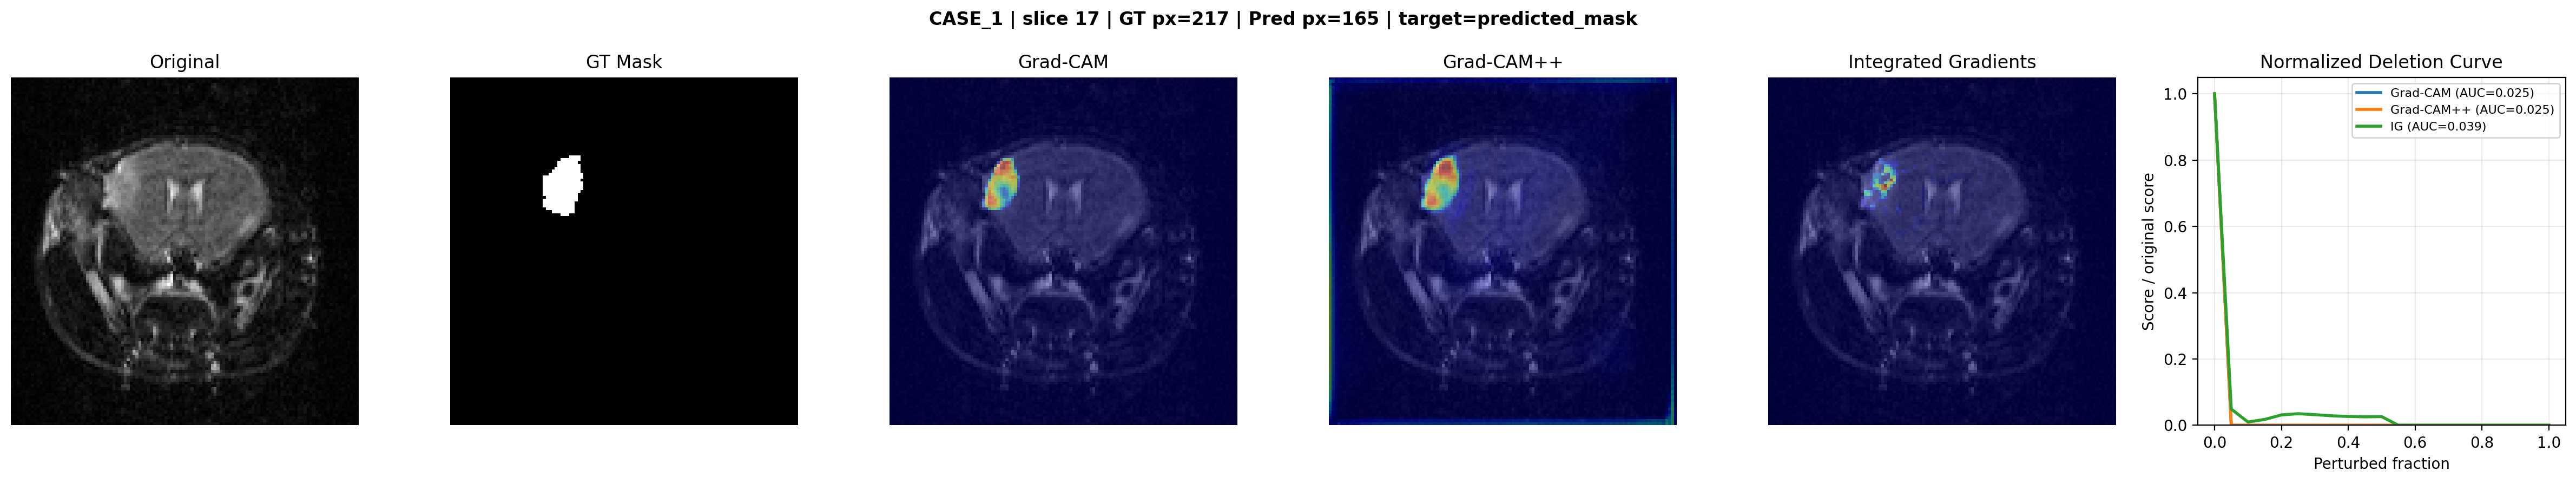
\includegraphics[width=\textwidth]{Imagenes/XAI_isquemia/CASE_1_slice_017.png}
    \caption{Ejemplo cualitativo de explicabilidad aplicado al modelo de segmentación de isquemia. Se muestran la imagen original, la máscara manual, la máscara predicha y los mapas de relevancia obtenidos mediante Grad-CAM, Grad-CAM++ e Integrated Gradients.}
    \label{fig:xai_isquemia_ejemplo}
\end{figure}

Este comportamiento resulta especialmente relevante en segmentación médica, donde una explicación coherente puede ayudar a identificar si el modelo se apoya en patrones anatómicos plausibles o en regiones ambiguas de la imagen.

La evaluación cuantitativa mediante perturbación, resumida en la Tabla~\ref{tab:xai_isquemia_resultados}, refuerza esta interpretación. En los cortes con lesión correctamente detectada, los valores medios de \textit{Deletion AUC} fueron muy bajos para los tres métodos, con valores de 0,025 para Grad-CAM y Grad-CAM++, y 0,026 para Integrated Gradients. Esto indica que, al eliminar en primer lugar las regiones consideradas más relevantes, el score asociado a la predicción cae de forma abrupta. De forma complementaria, las curvas de \textit{Insertion} muestran que al reconstruir la imagen empezando por las regiones más relevantes el modelo recupera progresivamente su activación, especialmente en Grad-CAM++ e Integrated Gradients, con valores medios de 0,840 y 0,879 respectivamente.

\begin{table}[H]
\centering
\caption{Resultados cuantitativos de explicabilidad para los cortes de isquemia correctamente detectados.}
\label{tab:xai_isquemia_resultados}
\setlength{\tabcolsep}{4pt}
\renewcommand{\arraystretch}{1.15}
\begin{tabular}{lcccc}
\hline
\textbf{Método} &
\makecell{\textbf{Deletion}\\\textbf{AUC}} &
\makecell{\textbf{Insertion}\\\textbf{AUC}} &
\makecell{\textbf{LeRF}\\\textbf{AUC}} &
\makecell{\textbf{AOPC}\\\textbf{normalizado}} \\
\hline
Grad-CAM & 0,025 & 0,627 & 0,867 & 1,000 \\
Grad-CAM++ & 0,025 & 0,840 & 0,840 & 1,000 \\
Integrated Gradients & 0,026 & 0,879 & 0,882 & 0,999 \\
\hline
\end{tabular}
\end{table}

Además, los valores de \textit{LeRF AUC} se mantienen elevados, lo que indica que al eliminar inicialmente las regiones menos relevantes la predicción se conserva durante una parte importante del proceso de perturbación. Del mismo modo, el \textit{AOPC} normalizado se sitúa en valores cercanos a 1 para los tres métodos, reforzando la idea de que las regiones destacadas por los mapas tienen una influencia significativa en la salida del modelo.

No obstante, el análisis también permite identificar limitaciones. En los falsos positivos, las explicaciones muestran activaciones localizadas en las regiones que han originado la predicción errónea. Esto evidencia que la explicabilidad no garantiza que la predicción sea correcta, sino que permite analizar qué información ha utilizado el modelo para producirla. Por tanto, estos casos resultan especialmente útiles para detectar patrones de error y posibles regiones ambiguas en la imagen.

En conjunto, los resultados de explicabilidad sugieren que el modelo de isquemia basa sus predicciones en regiones espacialmente coherentes con las máscaras generadas. Las técnicas Grad-CAM y Grad-CAM++ proporcionan explicaciones visualmente más compactas, mientras que Integrated Gradients ofrece una atribución más detallada pero menos localizada. La combinación de análisis cualitativo y métricas de perturbación permite aportar una capa adicional de interpretación al modelo, aunque sus resultados deben entenderse como apoyo a la evaluación del sistema y no como validación clínica independiente.

\subsection{Discusión crítica del modelo de isquemia}
Es importante destacar que el sistema desarrollado se concibe como una herramienta supervisada en la que el especialista mantiene el control de los datos finales. La herramienta permite la edición de cada una de las máscaras generada así como los valores volumétricos en cada corte de la resonancia analizada. Este enfoque garantiza que cualquier desviación pueda ser corregida de manera sencilla por el experto, integrando la automatización dentro de un \textbf{flujo de trabajo asistido y no sustitutivo}. 

\section{Conclusiones del capítulo}

De forma global, los resultados obtenidos muestran un comportamiento diferenciado entre las dos tareas abordadas. La segmentación cerebral presenta un rendimiento más estable y preciso, con métricas de solapamiento elevadas y errores volumétricos reducidos en todos los casos evaluados. Este resultado era esperable, ya que el cerebro constituye una estructura anatómica de mayor tamaño, con límites más definidos y menor variabilidad relativa entre sujetos.

Por el contrario, la segmentación de isquemia representa una tarea más compleja. Las regiones lesionadas son de menor tamaño, presentan bordes menos definidos y pueden mostrar una intensidad más variable en la imagen de resonancia magnética. Por ello, pequeñas discrepancias espaciales entre la predicción y la referencia manual tienen un impacto mayor sobre métricas como Dice o IoU. Aun así, el modelo permite localizar de forma coherente las zonas patológicas principales y proporciona estimaciones volumétricas útiles para una primera aproximación automatizada.

El análisis conjunto de métricas cuantitativas, resultados visuales y mapas de explicabilidad indica que la herramienta desarrollada cumple el objetivo de ofrecer apoyo al análisis de imágenes biomédicas, especialmente como sistema de asistencia y cuantificación preliminar. No obstante, los resultados también muestran que la segmentación de lesiones requiere una validación más amplia y un refinamiento adicional antes de su uso en contextos de análisis clínico o experimental más exigentes.

\begin{figure}[h]
    \centering
    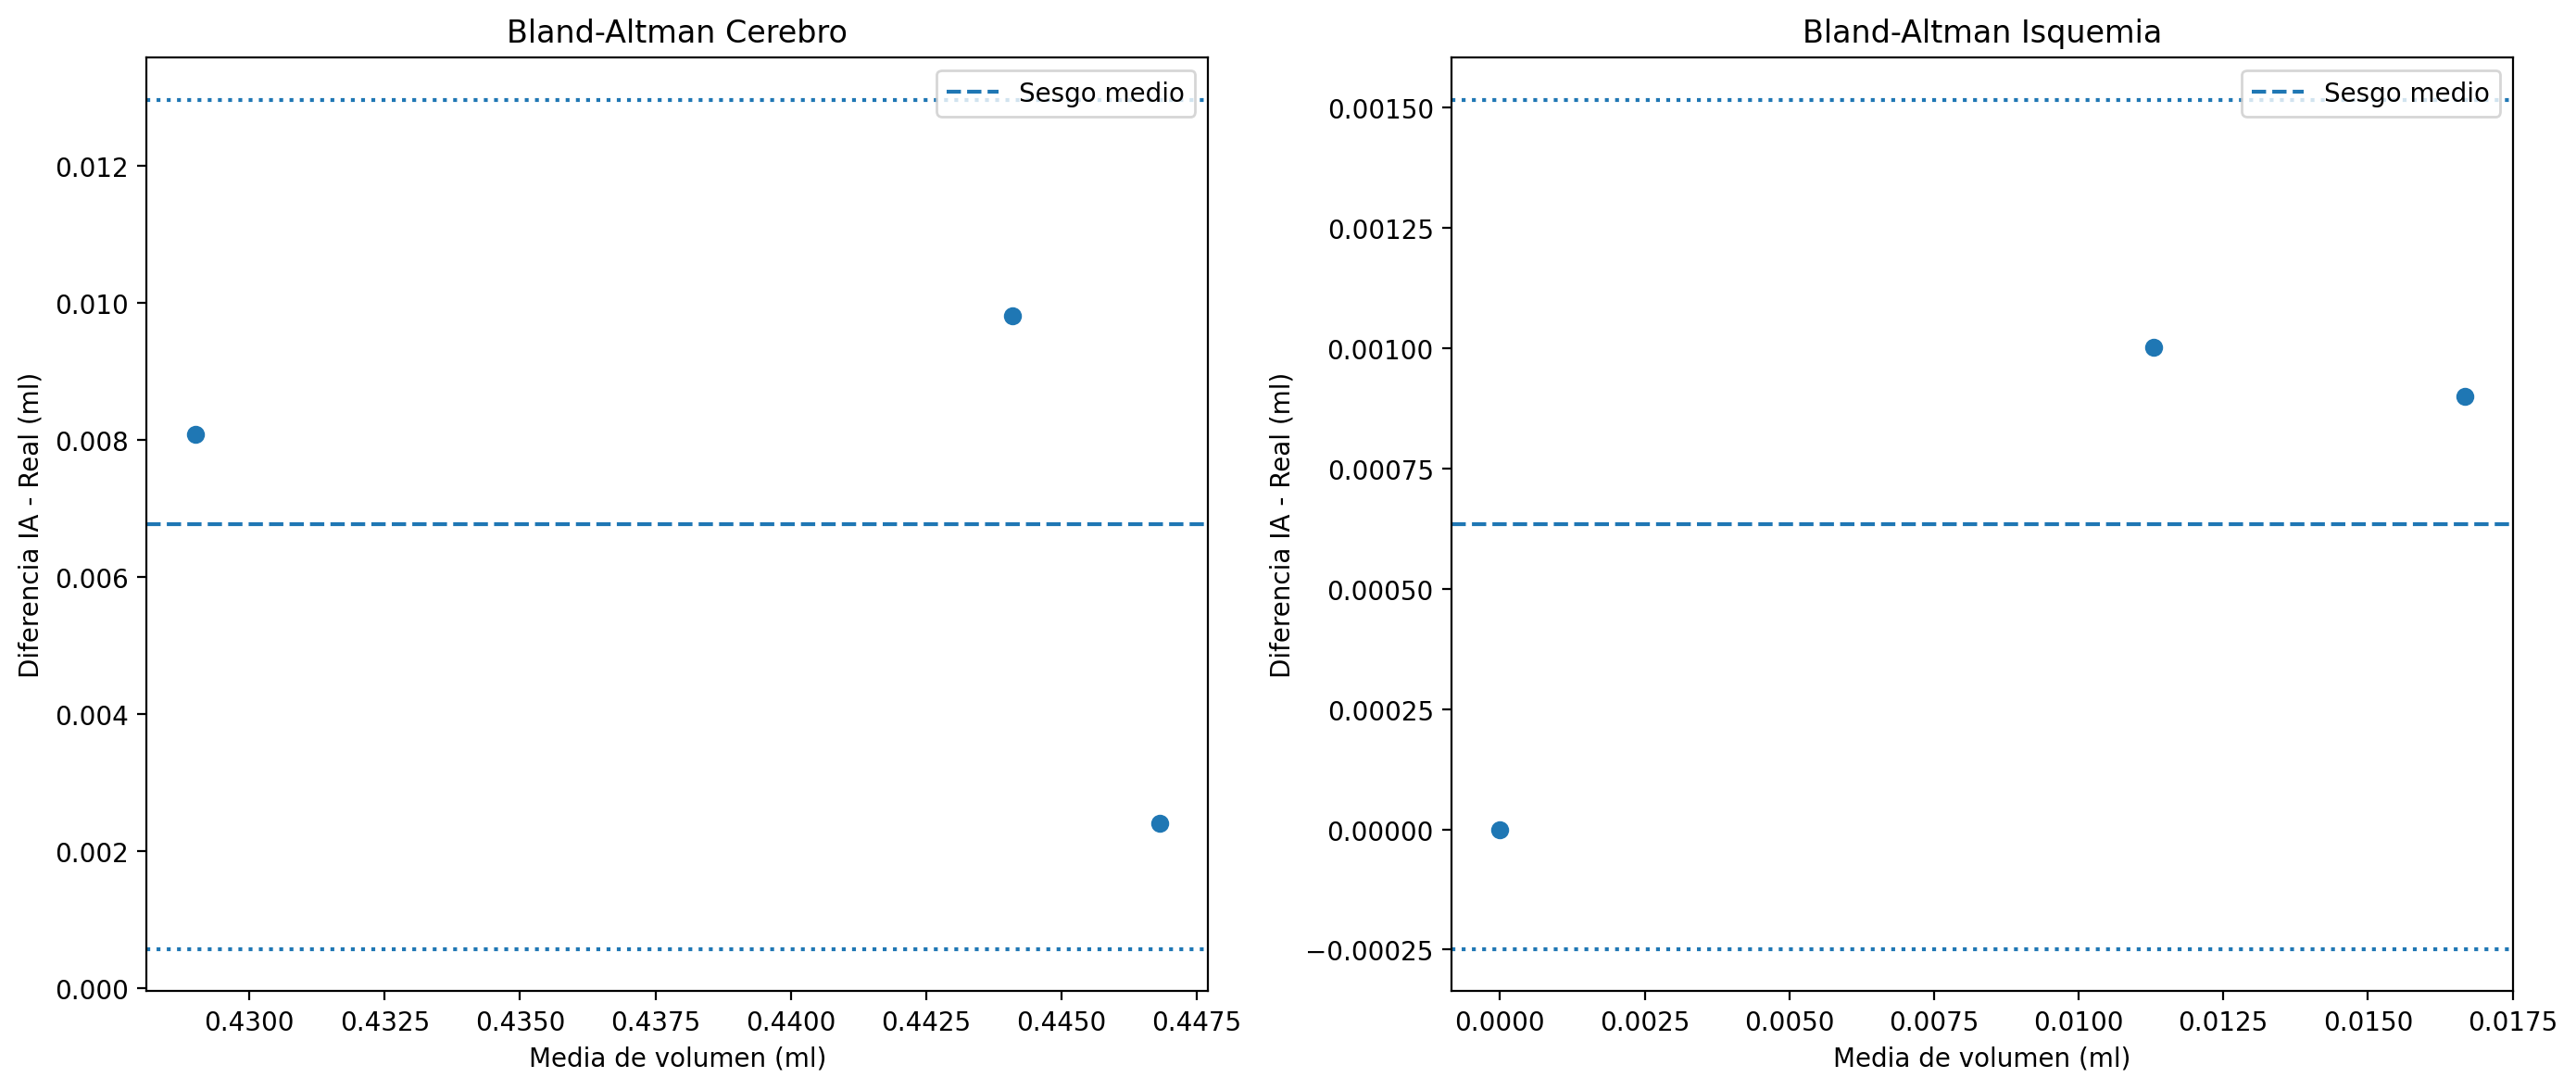
\includegraphics[width=1\textwidth]{Imagenes/Plots/bland_altman.png}
    \caption{Gráfico de Bland-Altman para analizar la concordancia entre el volumen real y el volumen estimado por el modelo.}
    \label{fig:bland_altman}
\end{figure}

\begin{figure}[h]
    \centering
    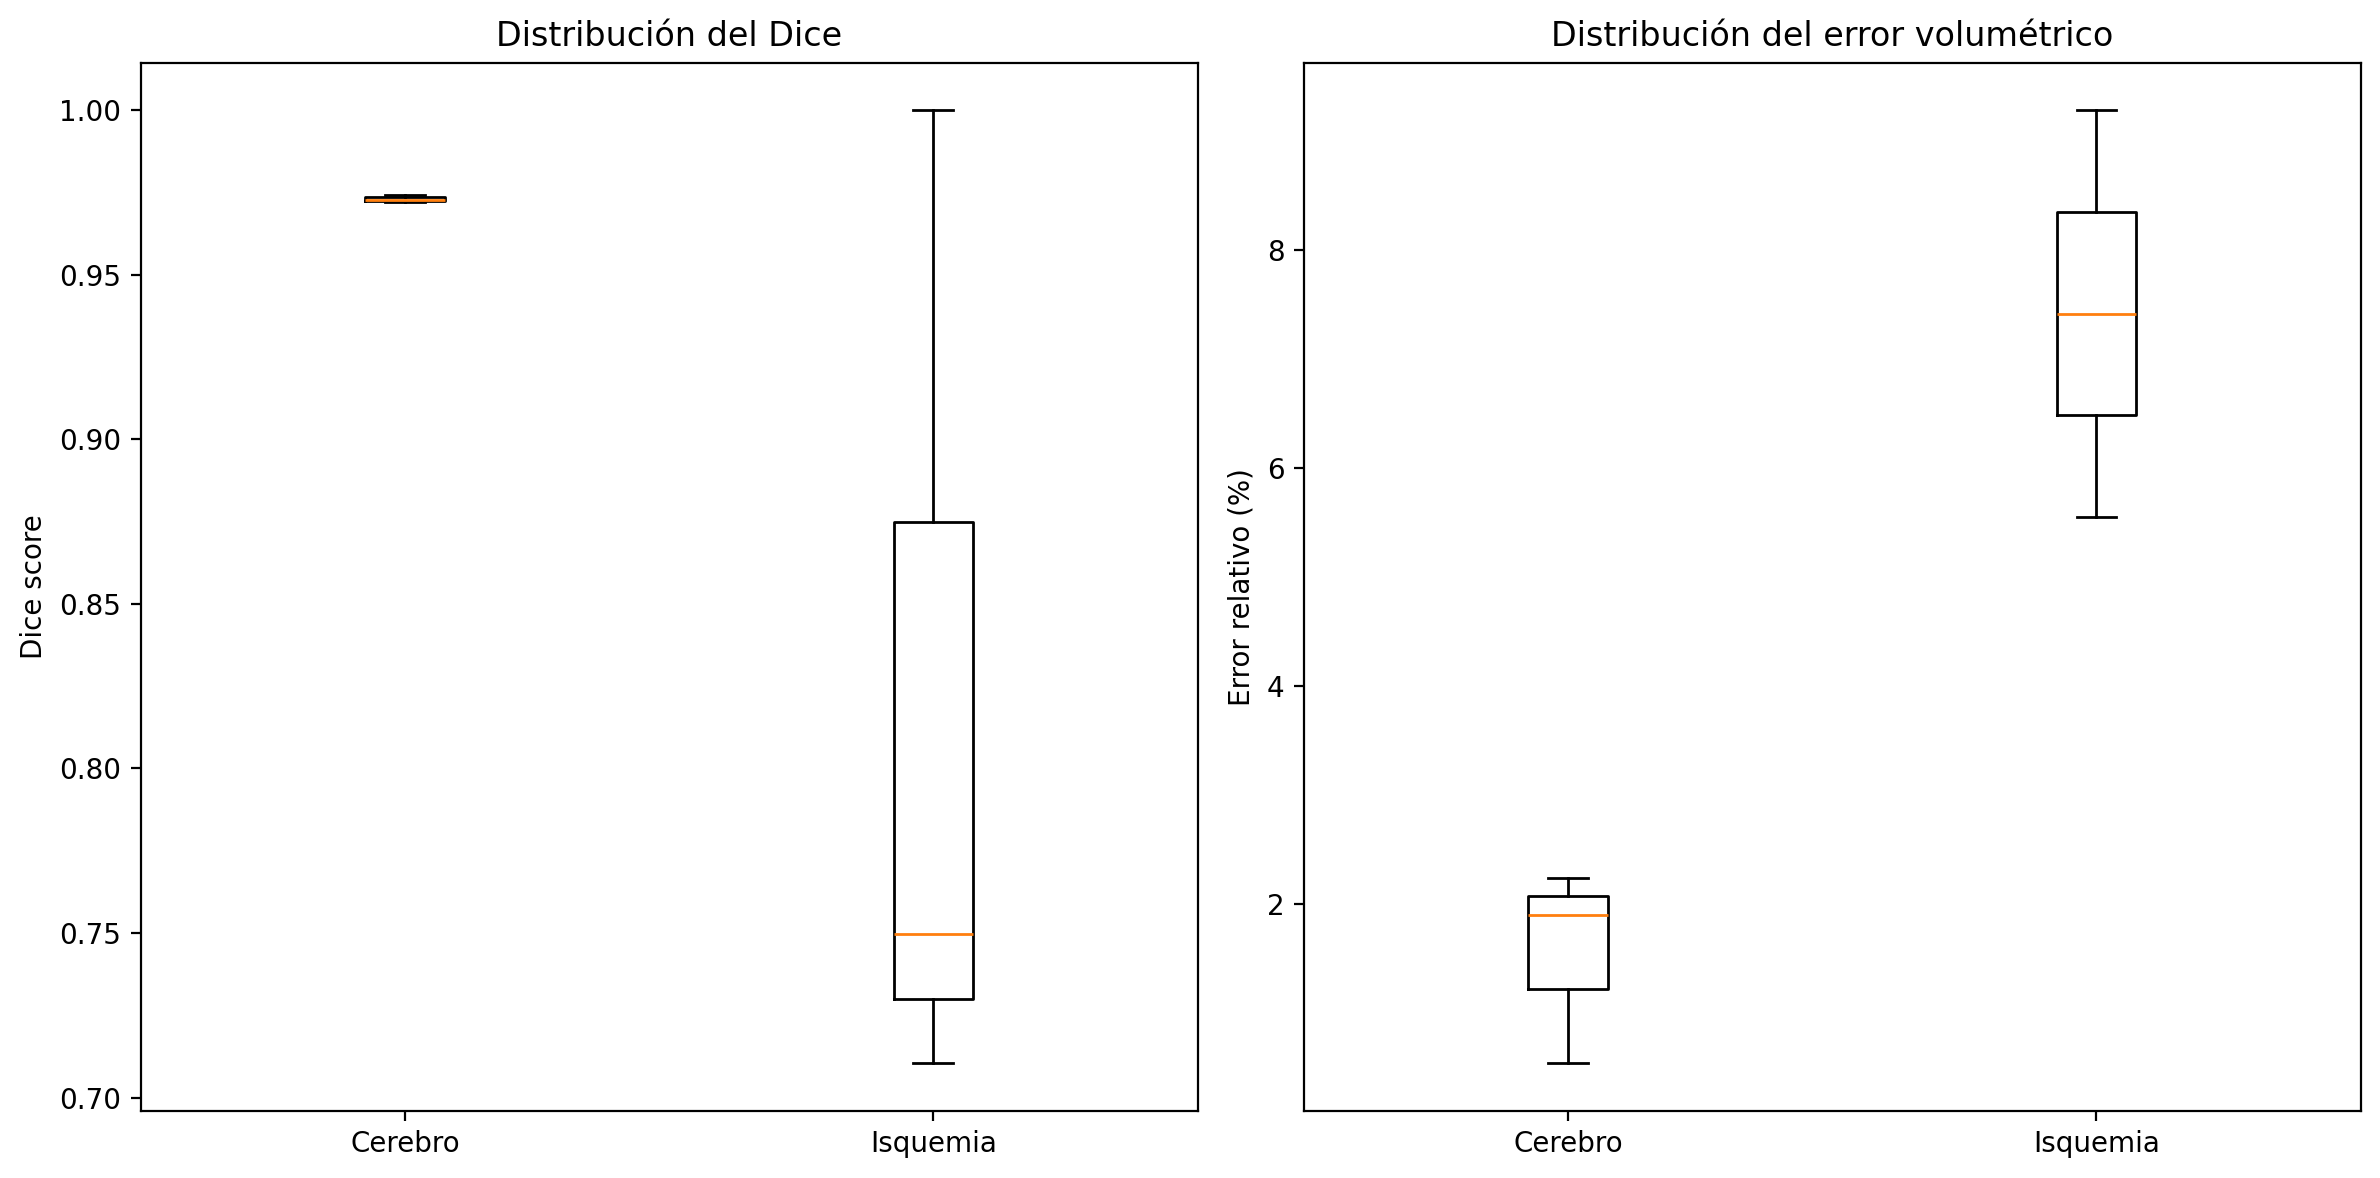
\includegraphics[width=1\textwidth]{Imagenes/Plots/boxplots_metricas.png}
    \caption{Distribución de las principales métricas de evaluación obtenidas en los casos analizados.}
    \label{fig:boxplots_metricas}
\end{figure}

\begin{figure}[h]
    \centering
    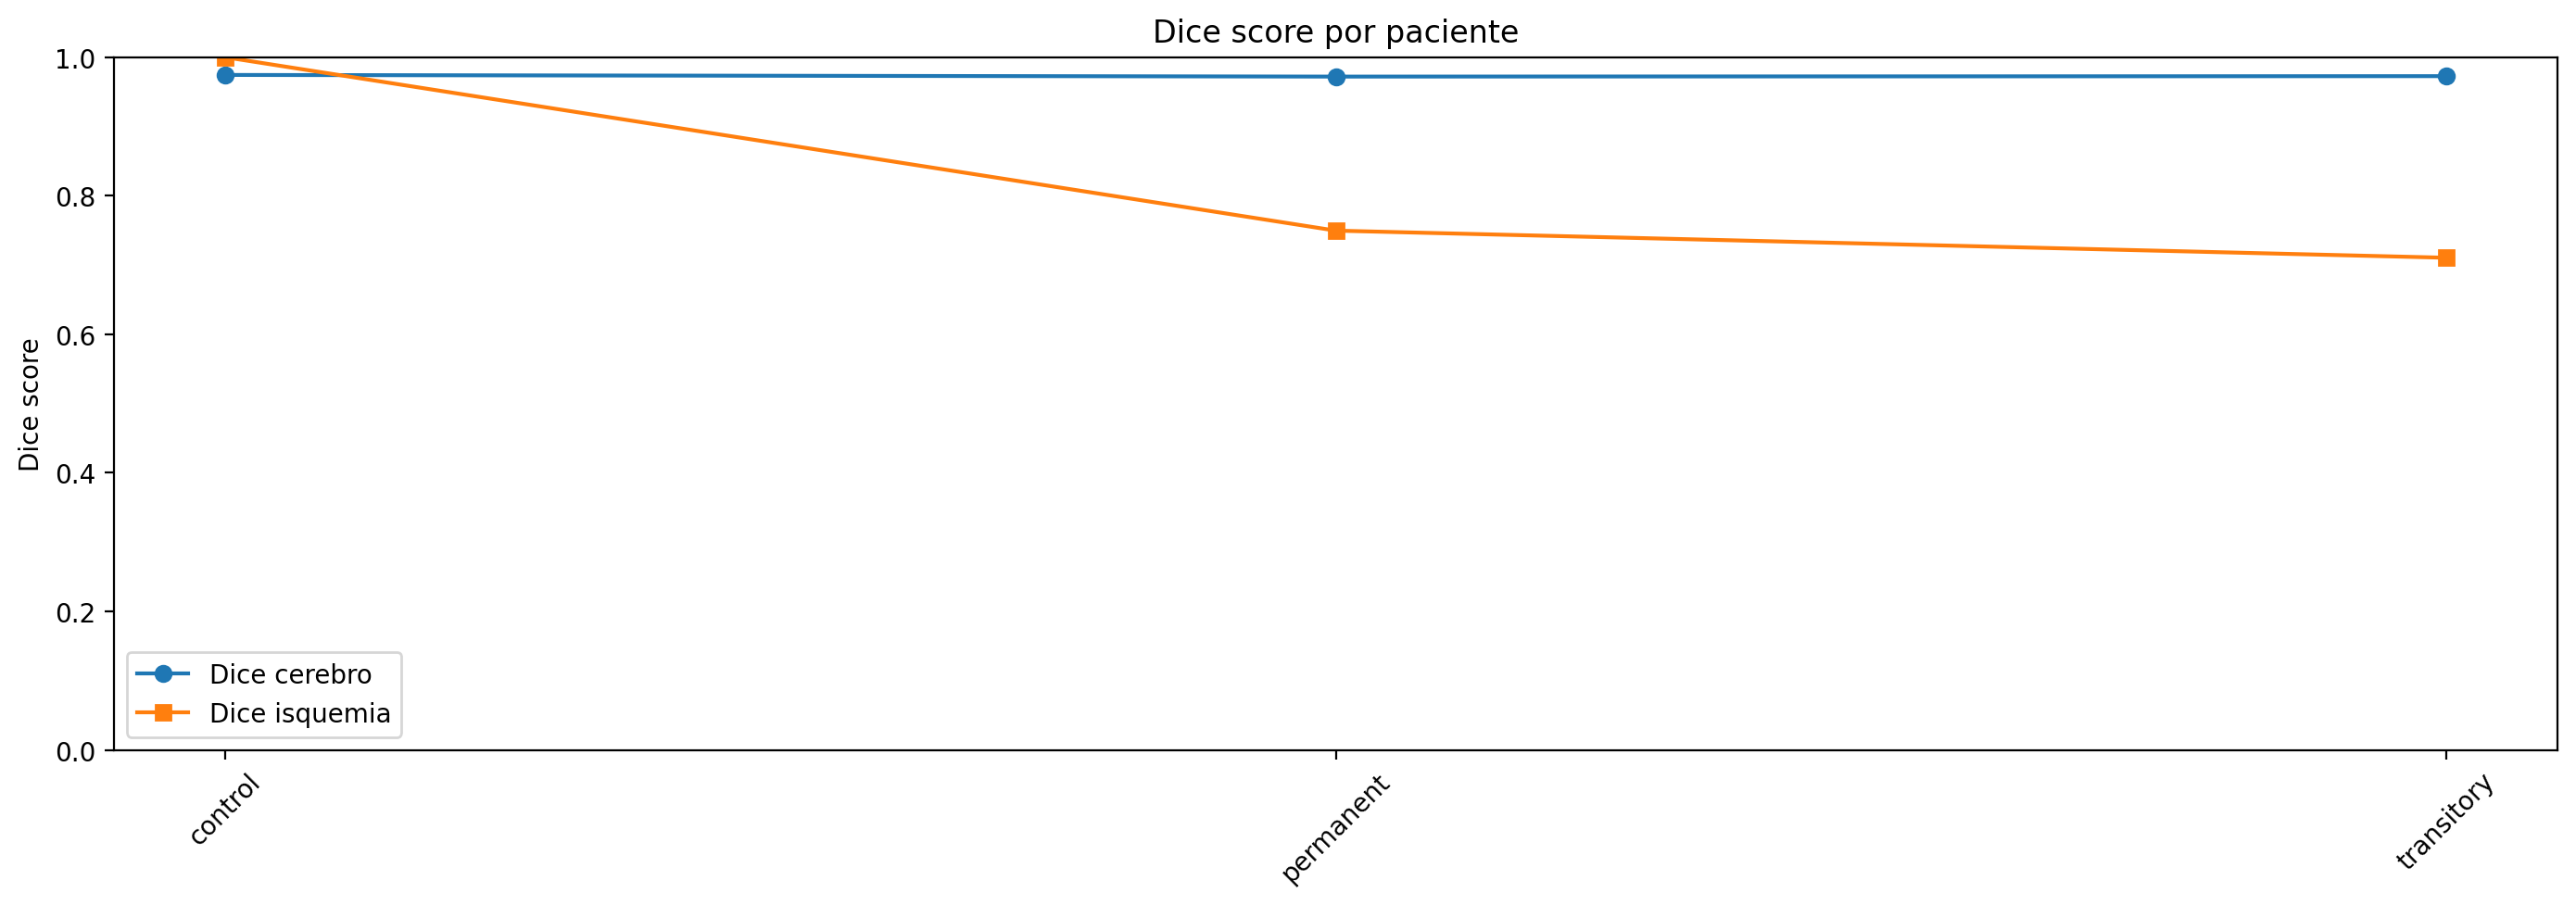
\includegraphics[width=1\textwidth]{Imagenes/Plots/dice_pacientes.png}
    \caption{Comparación del coeficiente Dice medio obtenido para cada paciente evaluado.}
    \label{fig:dice_pacientes}
\end{figure}